% Compile with XeLaTeX and the supplied APMCM class on TEXINPUTS.
\documentclass{apmcmthesis}
\usepackage{url}
\usepackage[section]{placeins}
\usepackage{needspace}
\usepackage[hidelinks,pdfauthor={},pdftitle={Screening Perovskites When All Exact Targets Are Hidden}]{hyperref}
\tihao{D}
\baominghao{}
\input{numbers.tex}
\renewcommand{\baselinestretch}{1.10}
\setlength{\parindent}{0pt}
\setlength{\parskip}{.45em}
\setlength{\headheight}{15pt}
\setcounter{tocdepth}{2}
\titleformat{\section}{\centering\normalfont\Large\bfseries}{\thesection.}{.5em}{}
\setlength{\emergencystretch}{1.2em}
\captionsetup{font=small,labelfont=bf,justification=raggedright,singlelinecheck=false}
\newcommand{\Vh}{\widehat V}
\newcommand{\noo}{\mathrm{NO}_2}
\newcommand{\ooo}{\mathrm O_3}
\newcommand{\foo}{\mathrm{FO}_2}
\newcommand{\subhead}[1]{\par\smallskip{\large\bfseries #1}\par\nopagebreak}
\begin{document}
\pagestyle{mainmatterstyle}
\begin{abstract}
\begin{center}
{\Large\bfseries Screening Perovskites When All Exact Targets Are Hidden}\\[3pt]
{\large A band-gap surrogate and an audited 8-bit QUBO search}
\end{center}
All 19 zero-violation compositions in the 18,928-candidate grid belong to the hidden set. We train on public records to predict violations for 3,703 hidden compositions and rank candidates for the next physical calculation. Every labeled zero-gap material has coincident band edges. Under the contest loss this implies a violation of at least 10.8658. We use a composition-based classifier to estimate the probability of a positive gap and fit separate violation regressions for the two regimes.

On 3,969 validation compositions from unseen element pairs, the resulting model retrieves 13 of the 27 materials with $V<1$ in its first 50 choices, compared with six for direct regression. A second seed gives 15 versus ten. In the three-family validation pool at seed 26, the top 50 contain five of eleven near-targets for the mixture and one for the 350-tree direct model (four with 1,050 trees). Both rank $\mathrm{InTiO_3}$ first. Its observed violation of 11.49225 exceeds the pool minimum of 0.04000 by 11.45225.

After refitting on all public labels, the full-pool surrogate selects $\mathrm{LaTiO_2N}$ for fixed $\noo$ ($\Vh=6.924382$) and $\mathrm{SnTiO_3}$ for the three-family problem ($\Vh=3.268113$). The first material's physical violation is unknown. The second has public $V=0.001419$ and was seen during refitting. Both blind pools select $\mathrm{LaTiO_2N}$.

Direct 8-bit conversion changes the best legal pair in all six whole-grid settings tested on the three-family score table. We partition the table into $4\times4$ blocks, encode each as a quadratic unconstrained binary optimization (QUBO) problem, solve it with the Kaiwu SDK on a CPU, and break ties using the original scores. All 338 block solves pass exhaustive feasibility and energy checks. In both full candidate pools, the block solver recovers the minimum of the frozen prediction table. Direct scans of those same scores take only microseconds. The larger uncertainty is the physical loss at a previously unseen composition.
\keywords{perovskite screening, grouped validation, band-gap mixture, QUBO, coefficient precision}
\end{abstract}
\clearpage
\tableofcontents
\clearpage
\section{What can be learned when every exact target is hidden?}
Castelli et al.\ screened cubic perovskites for light-driven water splitting \cite{castelli}. A composition with a suitable gap can still fail on band alignment or stability. Problem D combines these failures into one score and asks for a single composition in each of two search spaces \cite{contest}. We can check predictions at thousands of public compositions, yet none attains zero loss. Q1 therefore evaluates a composition-only predictor on labeled pairs and scores the hidden set. Q2 and Q3 refit that predictor on all public labels and select a single material from a fixed-family and a three-family pool, respectively.

For ordered sites $A$ and $B$ and anion family $X$, denote formation energy, GLLB-SC gap, valence edge and conduction edge by $e,g,v,c$, respectively, in eV. GLLB-SC is a computational approach to estimating band gaps \cite{kuisma}. We retain the edge convention in the supplied data. The five penalties represent excessive formation energy, a gap below or above its window, and a violation of either band-edge threshold. With $[t]_+=\max(0,t)$ and all energy scales in eV, the dimensionless contest loss is
\begin{align}
 d&=(e-0.21,\;1.4-g,\;g-3.1,\;5.73-v,\;c-4.50),\notag\\
 V(A,B,X)&=\sum_{j=1}^5 [d_j/0.5]_+^2. \label{eq:loss}
\end{align}
Equation~\eqref{eq:loss} includes equality in its zero set. The organizers report 19 compositions with $V=0$ and 15 under the strict physical inequalities. We use the former convention. Recomputing $V$ from the four rounded public quantities gives a maximum absolute discrepancy of $1.02\times10^{-5}$. We fit the supplied six-decimal target after this check.

The partitions in Table~\ref{tab:data} keep all seven anion families of each ordered pair together.

\begin{table}[htbp]
\caption{Official partitions. Each pair contributes seven families to its partition. The hidden exact-target count comes from the organizers.}\label{tab:data}
\centering\begin{tabular}{lrrrr}
\toprule Partition & Pairs & Rows & $V=0$ & $V<1$ observed\\\midrule
Training (02) & 1,608 & 11,256 & 0 & 83\\
Selection (03) & 567 & 3,969 & 0 & 27\\
Holdout (04) & 529 & 3,703 & 19 & unavailable\\\bottomrule
\end{tabular}
\end{table}

The grid contains $52^2\times7$ compositions, including $A=B$. The pair sets are disjoint. The seven families are O3, NO2, FO2, N2O, N3, O2S and FNO. File 06 repeats public compositions without labels. We use 02 for Q1 training, 03 for model selection and 04 for predictions. Q2 and Q3 use a separate fit on 02 and 03. The problem permits pools 07 or 11 for Q2 and 08 or 12 for Q3. We solve the full pools and separately identify the best candidates among unseen pairs. Sorting by identifier breaks exact score ties. Inference excludes identifiers, measured geometry and outcomes of density functional theory (DFT) calculations.

\subsection{Why A and B must remain ordered}
In the ideal cubic perovskite setting, place A at the corners, B at the body center and the anions at the face centers \cite{aflow}. The eight corners contribute $8/8=1$ A atom per cell. The six faces contribute $6/2=3$ anions. B has six nearest anion neighbors in the illustrated octahedron, while the periodically repeated face centers give A twelve nearest anion neighbors. The contest family label specifies the composition of the three anions. For example, NO2 supplies one N and two O per formula unit. The files give no site-resolved O/N ordering for the blind candidate.

Figure~\ref{fig:cell} holds the ideal fractional coordinates fixed while exchanging the cations. Each panel's gap and violation come from its own public DFT record.

\begin{figure}[htbp]
\centering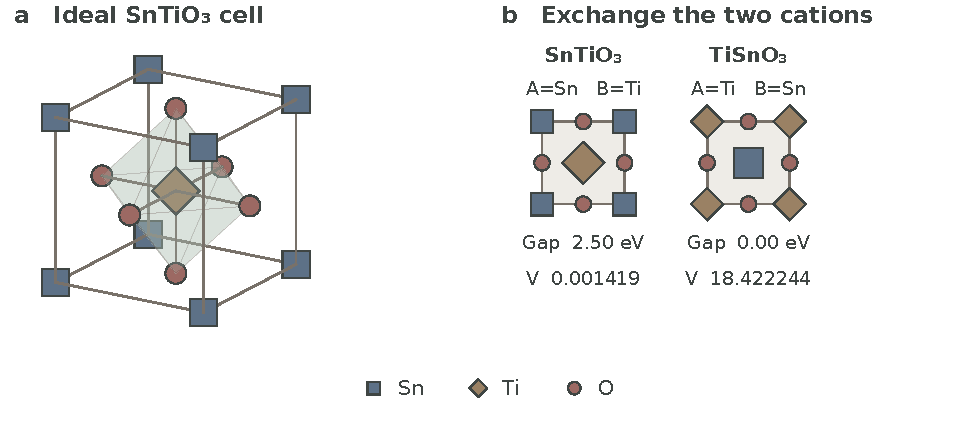
\includegraphics[width=.98\linewidth]{figures/crystal_sites.pdf}
\caption{Ordered sites in the ideal cubic prototype and two independently computed oxide records. In the unit cell Sn occupies the A corners and Ti the B center. The projected sections at right show the cations and equatorial oxygen sites. Squares mark Sn, diamonds Ti and circles O in both panels. Geometry follows the cubic prototype \cite{aflow}.}\label{fig:cell}
\end{figure}

We matched each public record $(a,b,x)$ with $(b,a,x)$ when both were labeled, excluded $a=b$, and counted each reciprocal pair once. Among 5,971 matches, the median absolute difference is 5.5296, with quartiles 2.2672 and 12.6046. A predictor that gives both records the same output $h$ incurs
\[
 \tfrac12\{|V(a,b,x)-h|+|V(b,a,x)-h|\}\ \geq\
 \tfrac12 |V(a,b,x)-V(b,a,x)|.
\]
Averaging the right-hand side gives an unavoidable MAE of at least 4.6805 on these 11,942 matched rows for a site-invariant predictor. This bound concerns the matched sample and must be compared on that same sample. It motivates retaining separate A and B descriptors before fitting.

The Sn--Ti pair illustrates the size of this effect. Public $\mathrm{SnTiO_3}$ has $g=2.50$ eV and $V=0.001419$. Its reversed assignment $\mathrm{TiSnO_3}$ has $g=0$ and $V=18.422244$. For $\mathrm{SnTiO_3}$ the supplied cubic lattice parameter is 3.969143~\AA. Lattice parameters and volumes are available only in labeled records and do not enter the score of a new composition.

\section{Problem 1. A lower bound for the metallic branch}
Of 15,225 public rows, 14,652 have $g=0$. On every one, $v=c$. Set both edges to $t$. The gap alone contributes $(1.4/0.5)^2=7.84$. Between 4.50 and 5.73, the two edge penalties form a convex quadratic symmetric about $t=5.115$. Outside that interval their sum increases. Formation energy can only add a nonnegative penalty. Hence under the observed coincident-edge convention
\begin{equation}
 V_{\rm metal}\ \geq\ L=7.84+
 \frac{(5.73-4.50)^2}{2(0.5)^2}=10.8658. \label{eq:metal}
\end{equation}
The smallest metallic values observed against the bound in Eq.~\eqref{eq:metal} are 10.865834 in training and 10.866614 in validation. A zero-gap record thus teaches the model where a near-target is physically unlikely. At prediction time the gap is unknown.

\subhead{Reading the lower bound in the public records}
The metallic lower bound resolves the gap and both edge penalties jointly. For a metal with common edge $t$, the vertical distance above the curve below equals the formation-energy penalty up to rounding.
\[
 B(t)=7.84+[ (5.73-t)/0.5 ]_+^2+[(t-4.50)/0.5]_+^2 .
\]
Moving the common edge to the left alleviates the CBM violation while increasing the VBM violation. Moving it to the right has the opposite effect. Their thresholds are separated by 1.23 eV. Figure~\ref{fig:regimes} shows why neither edge adjustment can compensate for zero gap.

\begin{figure}[htbp]
\centering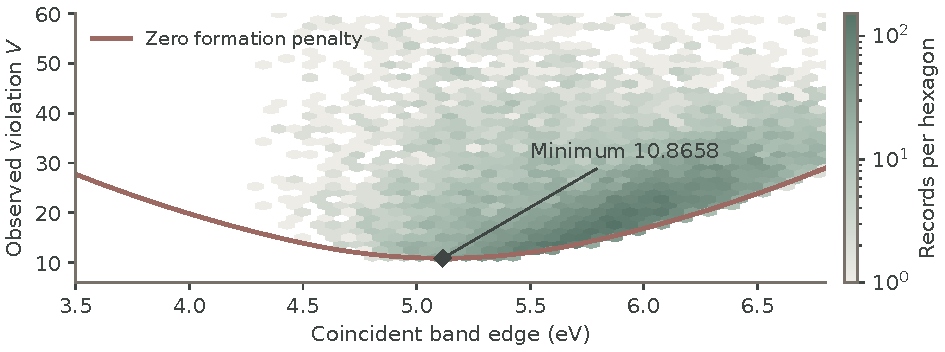
\includegraphics[width=\linewidth]{figures/physical_regimes.pdf}
\caption{Zero-gap records in files 02 and 03, grouped into hexagons in the displayed window. The color scale counts records. The curve gives the lower bound $B(t)$ and the diamond marks its minimum at $t=5.115$ eV.}\label{fig:regimes}
\end{figure}

Positive gap narrows the public screen from 15,225 records to 573 and retains all 110 with $V<1$. Even with the true gap known, only $110/573=19.2\%$ of the gapped records pass this relaxed test. In O3, 28 of 132 gapped compositions have $V<1$. In NO2, the ratio is 14 of 70, and in N3 none of 18 passes. These counts are descriptive. In particular, the hidden set was constructed to contain the exact targets, which changes the interpretation of any full-population prevalence estimate.


\subhead{A surrogate with observable training labels}
Composition-based descriptors have proved useful in inorganic property prediction \cite{ward}. For each metal site separately we use atomic number, Pauling electronegativity, periodic-table row and group from pymatgen \cite{ong}. Three categorical fields $A,B,X$ bring the total to eleven. This preserves site order and assumes the supplied cubic prototype throughout.

CatBoost handles the categorical inputs \cite{catboost}. Let $p(z)$ estimate $\Pr(g>0\mid z)$ from composition features $z$. Two regressors estimate $V$ conditional on positive and zero gap. The law of total expectation motivates
\begin{equation}
 \Vh(z)=p(z)\max(0,f_+(z)) + (1-p(z))\max(L,f_0(z)).
 \label{eq:mix}
\end{equation}
File 02 supplies 432 positive-gap and 10,824 metallic outcomes for fitting the gate. This classification label is observed even though the exact screening target never occurs in 02. Soft weighting keeps every candidate eligible. A composition receiving a high $p$ may still fail the band-edge or formation-energy requirements.

We compare with one direct regressor for $V$ using identical descriptors, 350 boosting iterations per component, depth 5, learning rate 0.08, four CPU threads and seeds 26 and 42. The mixture fits three components. Holding depth and descriptors fixed, we also fit direct regressors with 700 and 1,050 trees. The first budget matches the nominal training-row passes of the gate plus its two disjoint branches, and the second matches their total tree count. We carry seed 26 forward to use one fixed score table for both optimization problems. File 03 was reused for exploratory model selection. Its metrics describe development performance. The Q1 deliverable, \texttt{q1\_holdout.csv}, contains one composition-only prediction for each of the 3,703 hidden IDs.

\subsection{Following one composition through the predictor}
Consider $\mathrm{InTiO_3}$, the first-ranked seed-26 mixture candidate in the Q3 validation subset. Its actual zero gap is available only when we evaluate the prediction. During screening, the classifier puts probability 0.5426 on a positive gap. The two regressors then disagree by 9.3786 score units. Figure~\ref{fig:gate} traces the two weighted contributions in Eq.~\eqref{eq:mix} and compares their sum with the public DFT-derived loss.

\begin{figure}[htbp]
\centering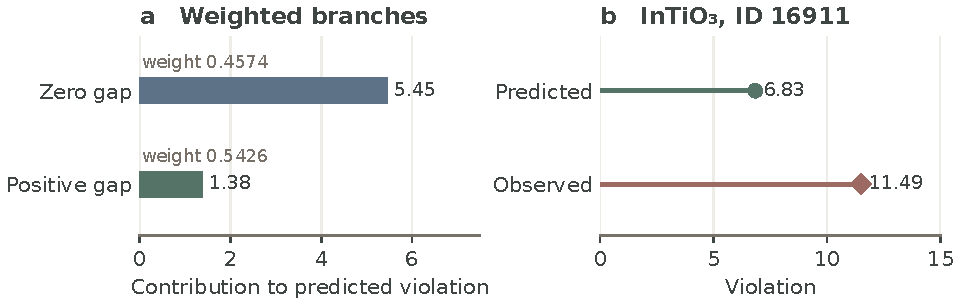
\includegraphics[width=\linewidth]{figures/gate_mechanism.pdf}
\caption{The composition-only gate for validation ID 16911 assigns positive-gap probability 0.5426. The bars give the contributions after weighting. The public loss was used only for evaluation.}\label{fig:gate}
\end{figure}

Writing $m$ and $u$ for the clipped metallic and positive-gap scores, respectively, gives $\Vh=m-p(m-u)$. The metallic branch contributes approximately $0.4574(11.9231)=5.45$ and the positive-gap branch $0.5426(2.5444)=1.38$. The arithmetic explains two features of this selection. First, a hard decision at $p=0.5$ would report only 2.5444, discarding a material portion of the expected violation. Second, a 0.10 increase in the positive-gap probability would lower the score by 0.938 with both branch estimates fixed. That sensitivity is large enough to matter among closely ranked candidates.

The gate also imposes a one-sided condition on very low scores. Since $u\geq0$ and $m\geq L$, Eq.~\eqref{eq:mix} gives
\[
 \Vh\geq (1-p)L,\qquad
 \Vh<1\ \Longrightarrow\ p>1-1/L\simeq0.9080 .
\]
This is a necessary condition on a \emph{predicted} score below one. A physically good but uncertain material may still receive a much larger score. Ranking by the continuous mixture keeps that material available when no candidate crosses a fixed prediction threshold. Conversely, assigning probability greater than 0.908 does not guarantee good band alignment or formation energy.

\subsection{A controlled test of the probability gate}
To isolate the effect of gating, we hold the learned branch functions $u$ and $m$, the seed, descriptors and train--validation split fixed. Only the mixing weight changes across the comparisons in Table~\ref{tab:gate}. The constant rule assigns the file-02 positive-gap fraction $432/11256$ to every composition. The hard rule replaces the predicted probability by $\mathbf{1}[p\geq0.5]$. The soft rule uses $p$ itself. A fourth, diagnostic rule routes each validation record by its observed gap label, an input unavailable on the blind pool. Replaying the soft rule reproduces all 3,969 archived validation scores within $10^{-8}$.

\begin{table}[htbp]
\caption{Changing only the gate on file 03. Hits count $V<1$ among the first 50. All-family and Q3 denominators are 27 and 11 available near-targets. The final column gives observed $V$ at Q3 rank one.}\label{tab:gate}
\centering\small\begin{tabular}{lrrrr}
\toprule Routing weight & All-family MAE & All hits & Q3 hits & Q3 first $V$\\\midrule
Training prevalence & 2.942 & 4 & 2 & 10.895\\
Hard decision & 2.909 & 8 & 1 & 11.492\\
Soft probability & 2.949 & 13 & 5 & 11.492\\
Observed gap (diagnostic) & 2.678 & 20 & 9 & 1.488\\\bottomrule
\end{tabular}
\end{table}

The hard decision gives a slightly smaller mean error than the soft mixture, yet it retrieves five fewer near-targets at budget 50 across all families. Many promising compositions fall below the hard threshold. Of the 141 validation materials with a positive gap, the classifier flags only 14 at $p\geq0.5$, alongside four false positives. Its precision there is $14/18$, while its recall is $14/141$. A hard rule makes the 127 missed positive-gap records share the metallic scoring regime with most of the validation set.

As a probability score for the positive-gap event, the gate attains a Brier score of 0.0273, compared with 0.0343 for the constant training prevalence. Average precision is 0.367 against a validation event frequency of 0.0355. These metrics assess the positive-gap event. No exact contest target occurs in the public labels. On Q3, even access to the observed regime yields a first choice with $V=1.4884$, above the near-target threshold. Improving the gate alone would still leave the regression problem of ranking positive-gap materials by their joint physical penalties.

\section{Validation at the actual screening budget}
For an ordered shortlist $S_k$ define $H_k=\sum_{i\in S_k}\mathbf1[V_i<1]$. Recall divides $H_k$ by the number of such targets in the relevant pool. For a one-choice decision $i^*$, labeled-pool regret is $R_1=V_{i^*}-\min_i V_i$. The expected number of $V<1$ hits in 50 random draws without replacement from the entire validation pool is $50(27/3969)=0.34$. Table~\ref{tab:val} compares this screening budget with the first-choice outcomes.

\begin{table}[htbp]
\caption{Performance on 567 unseen ordered pairs. Mean absolute error (MAE), root mean squared error (RMSE) and hits use all 3,969 rows. The last columns give observed $V$ at rank one in each restricted pool.}\label{tab:val}
\centering\small\begin{tabular}{lrrrrrrr}
\toprule Fit & Seed & MAE & RMSE & $H_{20}$ & $H_{50}$ & Q2 first & Q3 first\\\midrule
Direct &26&3.016&5.000&2&6&8.562&11.492\\
Mixture &26&2.949&4.828&8&13&10.927&11.492\\
Direct &42&3.013&4.945&3&10&11.540&46.240\\
Mixture &42&3.025&4.902&9&15&11.084&12.670\\\bottomrule
\end{tabular}
\end{table}

The mixture retrieves 48.1\% and 55.6\% of the 27 near-targets at $k=50$ for seeds 26 and 42. In Q2 it retrieves all four validation near-targets in 50 checks under both seeds, yet its first choice has $V>10$. In Q3, the seed-26 mixture and direct fits retrieve five and one of eleven near-targets. Both select $\mathrm{InTiO_3}$ first, with regret $11.49225-0.04000=11.45225$ (Figure~\ref{fig:screen}). Increasing the direct-model tree count to 700 and 1,050 raises its Q3 hit count from one to two and four at seed 26, with the same first choice. At seed 42 the counts are three, five and five, against six for the mixture. The shortlist advantage narrows as the direct model grows. The supplementary curves show both seeds and all pools (Figure~\ref{fig:allbudgets}).

\begin{figure}[htbp]
\centering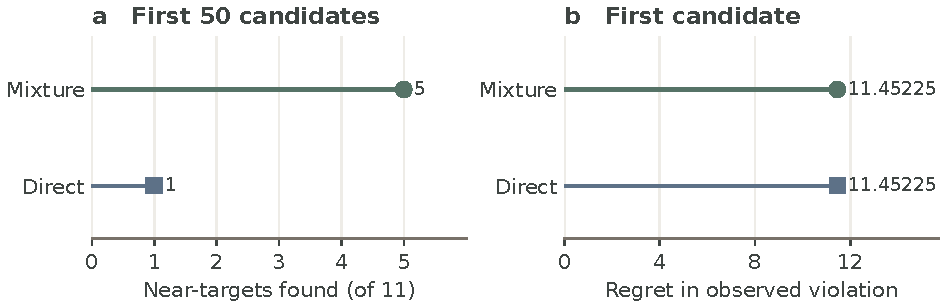
\includegraphics[width=.97\linewidth]{figures/q3_budget.pdf}
\caption{Screening at two budgets on the same 1,701 Q3 validation compositions, seed 26. Left, hits among the first 50, with a near-target defined by $V<1$. Right, the excess observed violation of the first choice over the attainable minimum.}\label{fig:screen}
\end{figure}

\subsection{How much of the shortlist survives a change of sample or seed?}
The validation sample contains 567 ordered metal pairs. Each pair contributes seven associated families, and we use the pair as the resampling unit. To assess sensitivity to the mix of pairs, we draw 567 pairs with replacement, retaining the whole family group and its multiplicity. On each resample we rank the records using the already fitted seed-26 predictors and count $V<1$ hits among the first 50. Figure~\ref{fig:stability} uses the same draw for both methods. This paired design preserves the dependence of their predictions on the same materials.

\begin{figure}[htbp]
\centering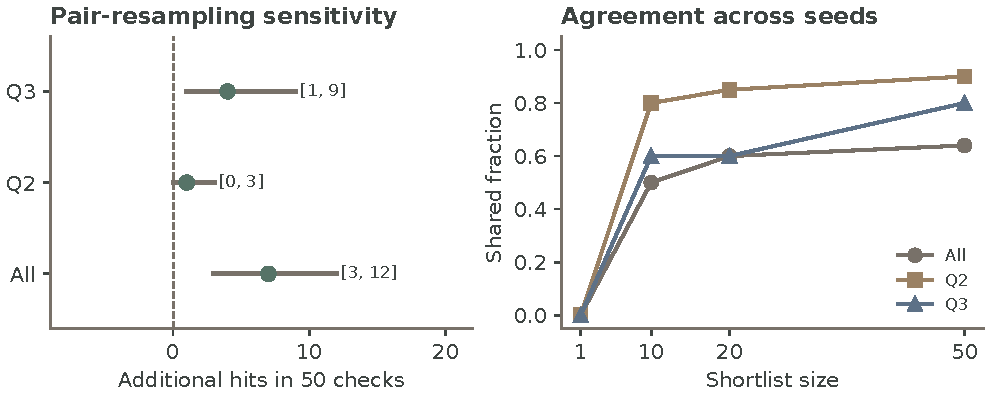
\includegraphics[width=\linewidth]{figures/validation_stability.pdf}
\caption{Left, observed mixture-minus-direct hit counts at budget 50 (dots) and the 2.5th to 97.5th percentiles over 2,000 resampled pair sets (segments). Right, the fraction of each mixture shortlist shared by training seeds 26 and 42 on the original validation set.}\label{fig:stability}
\end{figure}

Across all families the observed improvement is seven hits, with a resampling range of three to twelve. For Q2 the improvement is one and the interval reaches zero. Only four near-targets are present in that validation pool, leaving little room for a large observed gain. For Q3 the gain is four with a range of one to nine. The intervals describe sensitivity conditional on the trained models and the empirical pair distribution. Resampled duplicates count toward both hit totals and the 50-record budget. These are diagnostics of the metric, rather than prospective yields for 50 distinct new experiments.

We separately intersect the predicted shortlists from seeds 26 and 42. At $k=50$, 45 of 50 Q2 candidates and 40 of 50 Q3 candidates are shared. At $k=1$ the two seeds select different IDs in both pools. We therefore report the first choice on the frozen score table together with its validation regret. Seed agreement at a larger budget supports a follow-up shortlist but supplies little assurance about which single material a laboratory should measure first.

\section{Unseen pairs, withheld near-targets and a failed alternative}
We repeat the comparison inside file 02 with five shuffled folds of complete $(A,B)$ pairs. Each model uses four folds for fitting and ranks the fifth. Spending 50 checks in each held-out pool gives 250 checks per row of Table~\ref{tab:fold}. The five regrets describe variability across held-out compositions. The folds overlap in training data.
\begin{table}[htbp]
\caption{Five grouped folds within 02. The denominator counts all observed $V<1$ targets across the five held-out pools.}\label{tab:fold}
\centering\small\begin{tabular}{llrrr}
\toprule Pool & Method & Hits / targets & Median $R_1$ & Range of $R_1$\\\midrule
\FoldRows
\bottomrule\end{tabular}
\end{table}
In Q3 the mixture finds more near-targets over the five shortlists, yet its median first-choice regret is larger. A second stress test removes every pair containing $V<0.25$ from the training portion of file 02 and adds background pairs to form a 322-pair holdout. All 29 such targets lie among 2,254 held-out records. Across two background selections, direct regression retrieves five of 29 in its top 50 and the mixture retrieves nine. On the three-family subset the counts are five and seven of 20. Mixture rank-one $V$ moves from 13.8461 to 0.4756 while the attainable minimum is 0.0004 in both. These runs share the same targets. Their prevalence is 1.29\%, compared with 0.10\% for exact zeros on the contest grid.

\subhead{When predicting each physical quantity helps}
A public note suggested predicting the four physical properties first \cite{note1}. A second note discusses retaining metallic records for classification and regression \cite{note2}. Four separate 220-tree regressions predict $e,g,v,c$, followed by Eq.~\eqref{eq:loss}. At seeds 26 and 42, the property model selects a Q2 composition with observed $V=0.36$, versus 10.93 and 11.54 for a 220-tree direct fit. In Q3 both property fits choose $\mathrm{CaZrO_3}$ with $V=46.24$. At seed 26 its predicted gap is 2.19 eV, inside the window. The observed gap is 6.50 eV. The upper-gap term alone is $((6.50-3.10)/0.50)^2=46.24$. Average property accuracy conceals this error at the selected extreme. We carry the mixture forward for a common score table across both pools and its stronger shortlist performance. For a single Q2 choice, the property-first result favors that alternative on the available validation set.

\subsection{Reading a near miss and a false positive from their band edges}
The band-edge thresholds and gap window test different properties. Figure~\ref{fig:bands} compares the contest's two reported edges with their cutoffs and places the modeled and public gaps for $\mathrm{CaZrO_3}$ on a separate axis.

\begin{figure}[htbp]
\centering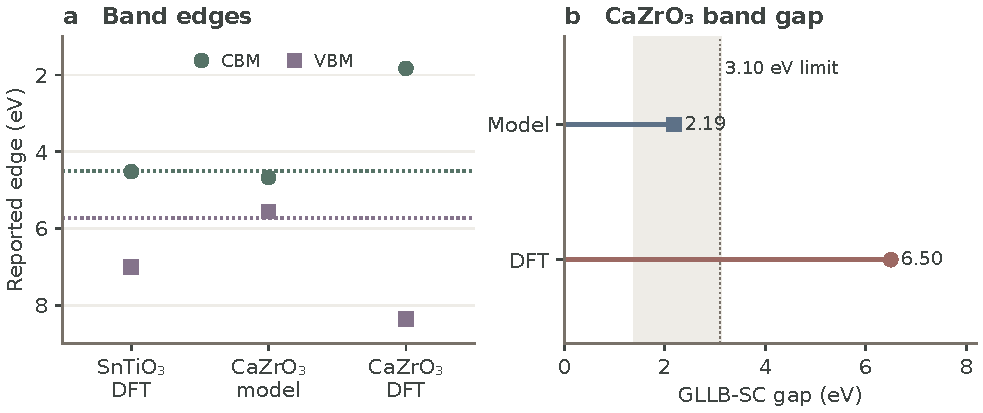
\includegraphics[width=\linewidth]{figures/band_edges.pdf}
\caption{Public DFT values and seed-26 property-model estimates. Left, the dotted lines mark the CBM (4.50 eV) and VBM (5.73 eV) cutoffs on the contest's inverted edge axis. Right, shading marks the 1.40--3.10 eV accepted gap interval.}\label{fig:bands}
\end{figure}

For $\mathrm{SnTiO_3}$, the CBM lies 0.018833 eV beyond its cutoff, a difference too small to resolve easily at the figure scale. For $\mathrm{CaZrO_3}$ the observed edges both pass, but the observed gap is 6.50 eV. It exceeds the upper limit by 3.40 eV and produces the entire observed violation of 46.24.

The modeled band edges help explain how the four-property model can rank that material first. It predicts $g=2.1883$ eV, with both small band-edge violations and a passing formation energy, for a total predicted $V=0.2342$. Its independently fitted edges imply $5.5559-4.6680=0.8879$ eV, far from its own gap estimate. In the public DFT record the analogous difference is 6.53 eV, close to the tabulated 6.50 eV. The discrepancy between the model's two estimates of the gap provides a composition-level warning that could be checked before spending a single assay. The following sensitivity test evaluates this warning across all Q3 validation pairs.

\subsection{Can a consistency check rescue a one-choice screen?}
The $\mathrm{CaZrO_3}$ failure suggests a testable diagnostic. Define
\[
 D(z)=\big|\hat g(z)-(\hat v(z)-\hat c(z))\big|.
\]
All three terms are predictions from the property-first model, so the diagnostic could be computed before measuring a candidate. It checks whether the two representations of the gap agree. A small residual can also occur when both representations are wrong in the same direction.

We test a veto on the 1,701 Q3 validation records. We discard predictions with $D>\tau$ and select the remaining candidate with the smallest property-first violation. Table~\ref{tab:veto} reports both seeds, with 26 first in each entry. The same 11 near-targets are available to each fit. Thresholds are exploratory, and this test does not alter the frozen mixture.
\begin{table}[htbp]
\caption{Cost of vetoing inconsistent property predictions. Entries give seed 26 / seed 42. Counts refer to distinct Q3 validation records.}\label{tab:veto}
\centering\small\begin{tabular}{lrrr}
\toprule Tolerance (eV) & Eligible records & Near-targets retained & First observed $V$\\\midrule
No veto & 1701 / 1701 & 11 / 11 & 46.24 / 46.24\\
1.00 & 1698 / 1699 & 11 / 10 & 11.25 / 46.24\\
0.50 & 1690 / 1681 & 10 / 9 & 11.97 / 11.25\\
0.25 & 1634 / 1623 & 7 / 5 & 11.97 / 10.88\\
0.05 & 753 / 805 & 0 / 3 & 10.88 / 10.93\\\bottomrule
\end{tabular}
\end{table}

At $\tau=0.50$ the large error on $\mathrm{CaZrO_3}$ is removed for both seeds, yet neither replacement is a near-target. At $\tau=0.05$ the seed-26 screen eliminates every available near-target. Agreement between model outputs can flag a case for inspection. Using that agreement as an automatic rejection criterion sacrifices some of the materials the screen is meant to find.



\section{Problems 2 and 3. Exact search on a finite score table}
\subhead{One representative of each metal site}
Let $a_i,b_j\in\{0,1\}$ indicate the selected A and B elements. For Q2 let $C_{ij}=\Vh(i,j,\noo)$. For Q3 store
\begin{equation}
 C_{ij}=\min_{x\in\{\ooo,\noo,\foo\}}\Vh(i,j,x),
 \qquad x^*_{ij}\in\arg\min_x\Vh(i,j,x).
 \label{eq:envelope}
\end{equation}
Taking $\min_{ij}$ in Eq.~\eqref{eq:envelope} visits every eligible triple. Recover $x^*_{ij}$ after choosing the pair, taking the smallest official ID in a tie. A joint one-hot encoding has 156 choices of $(A,X)$ and 52 choices of B. Eliminating X leaves 104 binary variables and a 2,704-cell table. It requires all 8,112 scores in advance. Solving three separate fixed-X problems is another exact decomposition.

For either real cost table, let $D$ denote its min--max normalization. The exactly-one penalty formulation \cite{lucas} is
\begin{equation}
 E(a,b)=\sum_{ij} D_{ij}a_i b_j+
 P\left[\left(\sum_i a_i-1\right)^2+\left(\sum_j b_j-1\right)^2\right].
 \label{eq:qubo}
\end{equation}
Each legal vector activates one cell. Each illegal vector has penalty at least $P$ and nonnegative table cost, so $P>1$ separates it from every legal state before rounding. The encoding represents any predictor evaluated on this finite pool. Requiring the fitted predictor itself to be quadratic would impose an unnecessary restriction.

\subhead{What changes at eight bits?}
Kaiwu converts linear fields to couplings with a reference spin, producing 105 Ising dimensions. The special-purpose quantum computer (SPQC) interface specifies signed 8-bit integer couplings \cite{sdk}. We convert Eq.~\eqref{eq:qubo} to Ising, apply the SDK precision adjustment at eight bits, convert back, and compare energies of all 2,704 legal states. We scan $P=1.1,3,10$ using the full Q3 envelope and a version capped at its tenth percentile before normalization. Both tables have the same original minimizer. Figure~\ref{fig:precision} compares the excess score on the unrounded table at each setting.

\begin{figure}[htbp]
\centering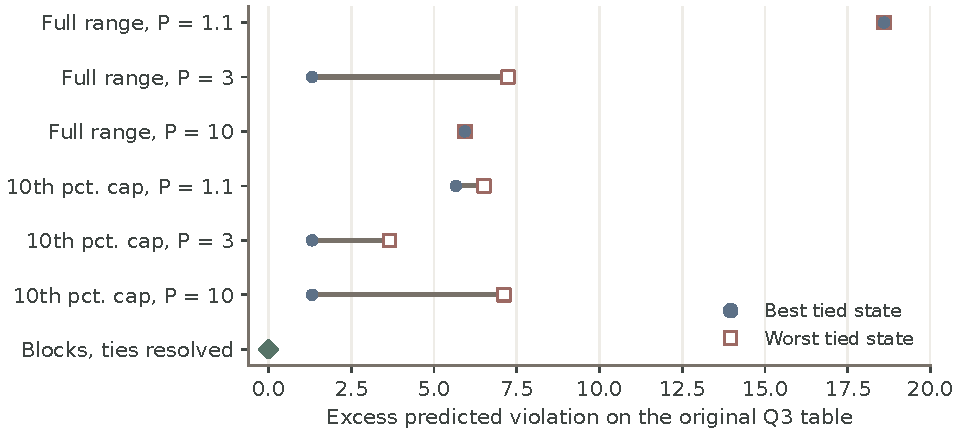
\includegraphics[width=.92\linewidth]{figures/precision.pdf}
\caption{Q3 original-score excess among legal states minimizing each quantized whole-grid energy. A segment spans tied outcomes. Coincident endpoints indicate identical excess. The diamond gives the verified result of the block method.}\label{fig:precision}
\end{figure}

\section{An eight-bit encoding with a checkable minimum}
All six whole-grid configurations in Figure~\ref{fig:precision} lose the minimum of the frozen mixture. For the full range and $P=1.1$, the winning legal pair costs an extra 18.5949 units of $\Vh$. A cap and $P=3$ reduce the best tied excess to 1.3175, still above zero. This audit checks only legal states. We now construct smaller blocks whose entire unconstrained state spaces can be checked.

Sort A and B alphabetically and partition each into thirteen consecutive groups of four. Each of the resulting 169 blocks $T$ covers 16 pairs. Let $M=\max_{ij\in T} C_{ij}$. For nonnegative costs use
\begin{equation}
 q_{ij}=\operatorname{round}(15C_{ij}/M),\quad
 q_{ij}\in\{0,\ldots,15\},\qquad P=16. \label{eq:bins}
\end{equation}
If $M=0$ set the whole block to zero. Use $q$ in Eq.~\eqref{eq:qubo}. A legal state has energy at most 15, whereas every illegal state costs at least 16. Rounding is monotone: the original block minimum is among the rounded minima. Retrieve the complete set of tied minima, read their original costs and keep the least. Comparing the 169 retained original costs recovers the global minimum. This proof depends on retrieving every ground state in a tied block. A sampler returning one arbitrary optimum has a weaker guarantee.

\subhead{Why the coefficients fit}
Write the upper-triangular QUBO with diagonal $-16$, within-group interactions $32$ and cross-group interactions $q_{ij}$, omitting the common constant 32. For eight bits $z$, set $s=2z-1$ and use one reference spin. With Kaiwu's $-s^\mathsf{T}Js$ convention, multiplying the returned symmetric matrix by eight gives integral couplings. Within-group entries are $-32$, cross-group entries are $-q_{ij}$. Each reference coupling is
\begin{equation}
 -\left(2(-16)+3(32)+\sum_{k=1}^4 q_{ik}\right)
 =-\left(64+\sum_{k=1}^4 q_{ik}\right), \label{eq:refcoupling}
\end{equation}
using the corresponding column sum on the B side. Equation~\eqref{eq:refcoupling} bounds its magnitude by 124. This is an a priori 8-bit bound for every block, independent of the absolute units of $\Vh$.

Kaiwu's \texttt{BruteForceOptimizer} solves the resulting nine-spin instances on the local CPU. We fix the gauge by multiplying every spin by the reference spin and deduplicate binary states. An independent pass checks all $2^8=256$ assignments in each block, including infeasible assignments. It verifies the affine energy relation, counts ground states, and compares every decoded optimum with the integer-cost table. Across both pools all 338 calls return complete sets of feasible ground states. Every retained block winner also matches the minimum of its original floating-point block.

\subhead{Why use four elements on each side?}
For a block of $n$ rows and $n$ columns with integer costs in $[0,K]$, the reference coupling of one logical variable has magnitude bounded by
\[
 B(n,K,P)=2P(n-2)+nK,\qquad n\geq2 .
\]
The $n-1$ same-register partners each contribute $2P$ and the diagonal contributes $-2P$ inside the reference term. Each of the $n$ cross-register partners contributes at most $K$. With $P=16$, $K=15$, blocks of side three, four and five have respective bounds 77, 124 and 171. Four is the largest uniform side length guaranteed to fit signed eight-bit couplings under this integer scaling. A particular five-element block may fit if its row and column sums are small. The uniform construction eliminates that data-dependent assumption.
\subsection{A worked example of an integer-energy tie}
Consider a Q3 block whose rows are Ir, K, La and Li and whose columns are Ge, Hf, Hg and In. In Figure~\ref{fig:tile} we select this block because, among the 169 Q3 blocks it has the largest spread of original scores tied at the lowest integer cost. It illustrates the cost of returning a single arbitrary ground state when the solver can return the whole tied set.

\begin{figure}[htbp]
\centering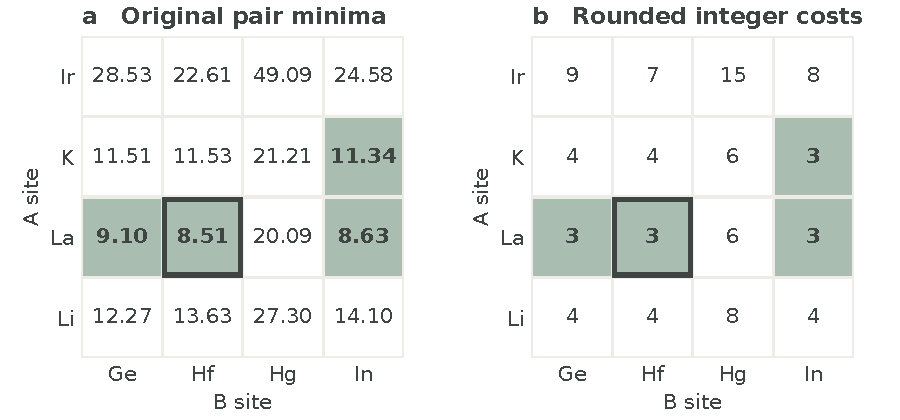
\includegraphics[width=.91\linewidth]{figures/tied_block.pdf}
\caption{The same Q3 block before and after Eq.~\eqref{eq:bins}. Shaded, bold cells share the lowest integer cost. The dark outline marks La--Hf, the original minimum. K--In ties after rounding but has an original score 2.82808 units higher. Displayed raw costs are rounded to two decimals after the calculation.}\label{fig:tile}
\end{figure}

The largest score in this block is 49.089358. The spacing of one integer bin is consequently about $49.089358/15=3.2726$ score units. Four pairs occupy the lowest bin. Their original scores are 8.511569 for La--Hf, 8.629274 for La--In, 9.102727 for La--Ge and 11.339649 for K--In. Each pair already carries its own minimizing $X$ from Eq.~\eqref{eq:envelope}. Selecting K--In would sacrifice 2.828081 units despite reaching the same minimum integer energy. Reading back the four original values returns La--Hf.

This example explains the difference between feasibility and selection accuracy. The penalty $P=16$ certifies one A and one B for every ground state in this block. It cannot distinguish the four shaded cells in Figure~\ref{fig:tile}. The monotonicity argument only places the best real-valued candidate somewhere among them. Full ground-state retrieval plus the original-score comparison is the additional condition needed for equality with the floating-point block minimum.

Integer minima tie in 70 of 169 Q3 blocks and 71 of 169 Q2 blocks. Choosing the highest original score among tied minima in every block gives the same two global winners in these runs because each winning block has a single minimizer. The largest within-block losses under this rule are 2.828081 for Q3 and 3.013807 for Q2. The cost breakdown includes time spent decoding and resolving ties.

\section{Selected compositions and computational cost}
Table~\ref{tab:answers} reports the single selections for Q2 and Q3 and the corresponding blind-pool checks.
\begin{table}[htbp]
\caption{Answers and membership checks. The two full pools are solved by Kaiwu. Direct scans of the two blind subsets give the restricted-pool comparison.}\label{tab:answers}
\centering\small\begin{tabular}{llrllrr}
\toprule Task & Pool (size) & ID & $(A,B,X)$ & Formula & $\Vh$ & Public $V$\\\midrule
Q2 & 07 (2,704)&13153& La, Ti, NO2 & LaTiO$_2$N & 6.924382 & hidden\\
Q3 & 08 (8,112)&8760& Sn, Ti, O3 & SnTiO$_3$ & 3.268113 & 0.001419\\\midrule
Q2 & 11 (529)&13153& La, Ti, NO2 & LaTiO$_2$N & 6.924382 & hidden\\
Q3 & 12 (1,587)&13153& La, Ti, NO2 & LaTiO$_2$N & 6.924382 & hidden\\\bottomrule
\end{tabular}
\end{table}
All four winners use the same refitted model. The ordered triplets explain why the file's NO2 family is written as O$_2$N in the supplied formula. For Q2 and Q3, respectively, runner-up scores are 7.256664 and 3.904881. Enumeration gaps for the chosen records are zero. Their winning-block Ising energies under $-s^\mathsf{T}Js$ are $-702$ and $-724$. Constants and scales vary by block, so comparing those two energies would have no physical meaning. $\mathrm{SnTiO_3}$ belongs to file 02; its public value is an in-training observation after refitting. For a new DFT calculation in the blind pool, both objectives nominate $\mathrm{LaTiO_2N}$. The appendix compares its three anion choices (Figure~\ref{fig:families}).

\subhead{Reading the selected bits}
A low Ising energy becomes a material recommendation only after the binary state has been decoded and compared across blocks. Figure~\ref{fig:decode} follows the Q3 winner. Holding Sn and Ti fixed, the three family scores are 3.2681 for O3, 8.2041 for FO2 and 12.3445 for NO2. The envelope stores the first value together with the O3 family and original row ID 8760.

\begin{figure}[htbp]
\centering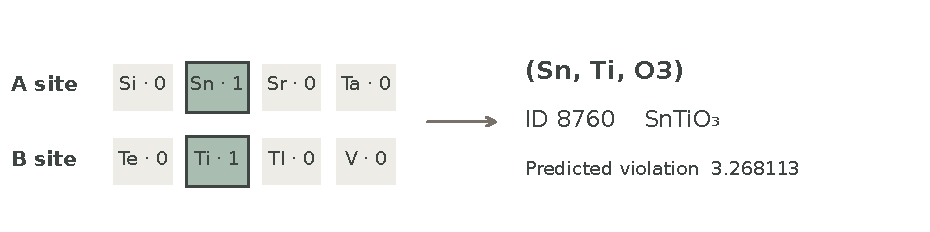
\includegraphics[width=\linewidth]{figures/qubo_decode.pdf}
\caption{Readout of the winning Q3 block. Each register contains exactly one active bit. Combining Sn and Ti with the stored minimizing family returns the full-pool material shown in Table~\ref{tab:answers}.}\label{fig:decode}
\end{figure}

The ordering $(\mathrm{Si,Sn,Sr,Ta})$ on A and $(\mathrm{Te,Ti,Tl,V})$ on B makes the second bit active in each register. If $\sigma_i$ is a returned spin and $\sigma_r$ the reference spin, the implemented readout is
\[
 z_i=\tfrac12(1+\sigma_i\sigma_r).
\]
Simultaneously reversing every spin leaves every product unchanged. The two gauge representations therefore identify the same pair and should be counted once. Fixing the reference to $+1$ gives binary vectors $(0,1,0,0)$ on both sides. The winning state's measured SDK energy is $-724$ and the decoded raw score is 3.268113. The block's lowest integer cost has one legal pair. Other blocks have different scale factors and omitted constants; their winners enter the final comparison through their raw scores.


Table~\ref{tab:cost} separates shared fitting and scoring costs from the pool-specific solver and scan times.

\begin{table}[htbp]
\caption{Wall-clock measurements on an AMD Ryzen 9 8945HX CPU. Fitting the three-component model is shared across both optimization problems.}\label{tab:cost}
\centering\small\begin{tabular}{lrr}
\toprule Stage & Q2 & Q3\\\midrule
Descriptors, shared (s) & \multicolumn{2}{c}{\DescFull}\\
Refit on 15,225 rows, shared (s) & \multicolumn{2}{c}{\FitFull}\\
Score 8,112 rows, shared (s) & \multicolumn{2}{c}{\ScoreFull}\\
Subset, index and reduce pool (s) & \PoolTwo & \PoolThree\\
Construct and convert 169 blocks (s) & \EncodeTwo & \EncodeThree\\
169 Kaiwu CPU solves (s) & \SolveTwo & \SolveThree\\
Decode, resolve ties, verify (s) & \CheckTwo & \CheckThree\\
Direct array minimum, median ($\mu$s) & \ScanTwo & \ScanThree\\
Blocks with ties / 169 & \TiedTwo & \TiedThree\\
Original costs compared within tied or unique minima & \FinalistsTwo & \FinalistsThree\\
Observed integer coupling range & $[\CoeffLowTwo,0]$ & $[\CoeffLowThree,0]$\\\bottomrule
\end{tabular}
\end{table}
The direct scan uses the same in-memory predictions and times 1,001 repetitions of one array minimum. The larger QUBO times include the checks itemized above; disk I/O and manuscript generation lie outside these timings. For Q1 alone, descriptors, training and scoring the hidden set took \DescOne, \FitOne\ and \ScoreOne\ seconds. These are local wall times under the observed machine load. Device programming, queueing, sampling, energy consumption and hardware success rates remain unmeasured.

\subsection{How much score error can change the recommendation?}
Checking the original score after decoding certifies the winner for a frozen table. Its robustness to changes in that table can be computed separately. Let $s_1<s_2$ denote the first two scores in one specified pool. If each score changes by at most $\epsilon$, the original winner remains strictly first whenever
\begin{equation}
 s_1+\epsilon<s_2-\epsilon
 \quad\Longleftrightarrow\quad \epsilon<(s_2-s_1)/2 .
 \label{eq:margin}
\end{equation}
The condition is sharp under independent bounded perturbations. Opposite changes at the two leading entries can create a tie at equality. If changes are correlated by composition, this worst case may be unattainable. Table~\ref{tab:margins} applies Eq.~\eqref{eq:margin} to each frozen pool. The resulting radii bound changes in predicted scores.

\begin{table}[htbp]
\caption{Selection margins in the archived Q2/Q3 refit. The last column counts records, including the winner, with predicted score at most two units above the minimum.}\label{tab:margins}
\centering\small\begin{tabular}{llrrr}
\toprule Pool & Runner-up & $s_2-s_1$ & Half-margin & Within 2 units\\\midrule
Q2 full (07) & $\mathrm{YTiO_2N}$ & 0.332282 & 0.166141 & 5\\
Q2 blind (11) & $\mathrm{YTiO_2N}$ & 0.332282 & 0.166141 & 2\\
Q3 full (08) & $\mathrm{GeTiO_3}$ & 0.636768 & 0.318384 & 5\\
Q3 blind (12) & $\mathrm{YTiO_2N}$ & 0.332282 & 0.166141 & 9\\\bottomrule
\end{tabular}
\end{table}

The two blind pools share a winner and runner-up because both leading NO2 pairs are eligible in either pool. Allowing the other two families raises the number of candidates within two score units from two to nine. More compositions can therefore enter a follow-up list even while the first two recommendations are stable to the change in pool. Conversely, expanding the Q3 blind pool to the full grid admits two public oxide candidates at the top. Reporting only the best score would conceal this change in the prospective experimental decision.

The unrounded full-pool Q3 half-margin is $0.318383852\ldots$ (displayed as 0.318384). Equality can produce a tie. Mean validation error gives no pointwise bound on a new material. The block algorithm addresses the first concern directly by comparing original scores for all integer ties. The material-selection risk remains governed by extrapolation to unseen pairs. For the next physical calculation, the score ledger identifies both the first candidate and its nearest competitor, while the grouped validation results quantify how often shortlists contain low-violation materials.


\section{Interpretation and limits}
Two kinds of error matter to a one-composition decision. For any returned candidate $u$ and a true minimizer $u^*$ in the same pool, adding and subtracting predicted scores yields
\begin{equation}
 V(u)-V(u^*)\ \leq\
 2\max_{z}|V(z)-\Vh(z)|+
 \underbrace{\Vh(u)-\min_z\Vh(z)}_{\text{optimization gap}} .
 \label{eq:regret}
\end{equation}
In Eq.~\eqref{eq:regret}, both extrema range over the specified pool. The optimization gap is zero in the two full pools. Mean validation error cannot bound the maximum score error at an unseen composition. On Q3 validation, exact minimization of the seed-26 surrogate still incurs physical regret of 11.45225.

The metallic bound transfers only to data with the same band-edge convention. Across the five unseen-pair folds, the mixture finds 23 of 50 three-family near-targets at 50 checks per fold, compared with 14 for direct regression. Its median single-choice regret is larger (13.521 versus 11.569). These results favor the mixture for a shortlist and leave uncertainty about its first choice.

The eight-bit construction preserves the score minimum when each block returns all ground states and their raw costs break ties. All candidates must first be scored, and a direct scan already finds the same minimum in microseconds. Any SPQC speed comparison still requires device success rates and end-to-end timings on matched inputs \cite{speed}.

The full-pool answers are $\mathrm{LaTiO_2N}$ for Q2 and $\mathrm{SnTiO_3}$ for Q3. For the next DFT calculation, both blind pools nominate $\mathrm{LaTiO_2N}$ (ID 13153, $\Vh=6.924382$). Its physical violation remains unknown.

\clearpage
\begin{thebibliography}{11}
\bibitem{castelli} Castelli I. E., Landis D. D., Thygesen K. S., Dahl S., Chorkendorff I., Jaramillo T. F., Jacobsen K. W., New cubic perovskites for one- and two-photon water splitting using the computational materials repository [J], Energy \& Environmental Science, 2012, 5, 9034--9043. \url{https://doi.org/10.1039/C2EE22341D}.
\bibitem{contest} APMCM Organizing Committee, Problem D: Application of Special Purpose Quantum Computer to Rare-Target Search in Perovskite Candidate Materials, official problem statement and accompanying dataset notes, 2026.
\bibitem{kuisma} Kuisma M., Ojanen J., Enkovaara J., Rantala T. T., Kohn--Sham potential with discontinuity for band gap materials [J], Physical Review B, 2010, 82(11), 115106. \url{https://doi.org/10.1103/PhysRevB.82.115106}.
\bibitem{aflow} AFLOW Encyclopedia of Crystallographic Prototypes, Cubic Perovskite (CaTiO$_3$) Structure, \url{https://aflow.org/p/AB3C_cP5_221_a_c_b-001/}, accessed 2026-11-26.
\bibitem{ward} Ward L., Agrawal A., Choudhary A., Wolverton C., A general-purpose machine learning framework for predicting properties of inorganic materials [J], npj Computational Materials, 2016, 2(1), 16028. \url{https://doi.org/10.1038/npjcompumats.2016.28}.
\bibitem{ong} Ong S. P., Richards W. D., Jain A., Hautier G., Kocher M., Cholia S., Gunter D., Chevrier V. L., Persson K. A., Ceder G., Python Materials Genomics (pymatgen): A robust, open-source python library for materials analysis [J], Computational Materials Science, 2013, 68, 314--319. \url{https://doi.org/10.1016/j.commatsci.2012.10.028}.
\bibitem{catboost} Prokhorenkova L., Gusev G., Vorobev A., Dorogush A. V., Gulin A., CatBoost: unbiased boosting with categorical features [C], Advances in Neural Information Processing Systems, 2018, 31, 6638--6648.
\bibitem{note1} Shumo Jiayouzhan, AI-assisted ideas for 2026 APMCM Problem D [translated title], Xiaohongshu, \url{https://xhslink.cn/o/5LxZKskY5UK}, accessed 2026-11-26.
\bibitem{note2} Shuxue Jianmo Laoge, A solution approach to 2026 APMCM Problem D [translated title], Xiaohongshu, \url{https://xhslink.cn/o/4SqQmBiyKO6}, accessed 2026-11-26.
\bibitem{lucas} Lucas A., Ising formulations of many NP problems [J], Frontiers in Physics, 2014, 2, 5. \url{https://doi.org/10.3389/fphy.2014.00005}.
\bibitem{sdk} QBoson, Ising matrix precision adaptation, Kaiwu SDK documentation, \url{https://kaiwu-sdk-docs.qboson.com/zh/latest/source/advanced/precision.html}, accessed 2026-11-26.
\bibitem{speed} R{\o}nnow T. F., Wang Z., Job J., Boixo S., Isakov S. V., Wecker D., Martinis J. M., Lidar D. A., Troyer M., Defining and detecting quantum speedup [J], Science, 2014, 345(6195), 420--424. \url{https://doi.org/10.1126/science.1252319}.
\end{thebibliography}

\clearpage
\section*{Appendix. Reproduction and complete source listings}
\phantomsection
\addcontentsline{toc}{section}{Appendix. Reproduction and complete source listings}
Python 3.12.14, CatBoost 1.2.10, pymatgen 2025.10.7, NumPy 2.5.5, pandas 2.2.3, SciPy 1.18.1, scikit-learn 1.9.1 and Kaiwu SDK 1.4.4 were used on Windows 11. Figures use the ideal cubic prototype, public physical properties, saved predictions and solver tables. The revised figures were rendered from the archived values with Matplotlib 3.10.8 and typeset with XeLaTeX and the APMCM class.

Place the original files in \texttt{problem\_d/date}. Run the data audit, the validation and stress comparisons for seeds 26 and 42, the physical-property comparison, the seed-26 encoding and precision audit, then the paper scripts. Running \texttt{screen.py scores} produces the hidden Q1 predictions and the refit Q2/Q3 score table. Running \texttt{screen.py development} produces the five-fold results. Use \texttt{solve.py} for both full-pool searches, \texttt{gate\_audit.py} for the gate replay, \texttt{capacity\_audit.py} for the direct-model controls and \texttt{mechanisms.py} for the consistency and margin checks. Run \texttt{figures.py}, \texttt{material\_figures.py}, \texttt{perovskite\_plates.py}, \texttt{crystal\_scenes.py} and \texttt{tables.py} for the manuscript. The companion README gives the arguments and file names for each call.

The score ledger records SHA-256 digests for the two exported tables. The block ledger contains the selected ID, tie count, integer-energy minimum, scaled Ising energy, observed coupling range and timing for each call. Both final-pool selections can be reconstructed from the tables alone.

\setcounter{figure}{0}
\renewcommand{\thefigure}{A\arabic{figure}}
\renewcommand{\theHfigure}{supp.\arabic{figure}}
\subhead{Screening curves by candidate pool}
\begin{figure}[htbp]
\centering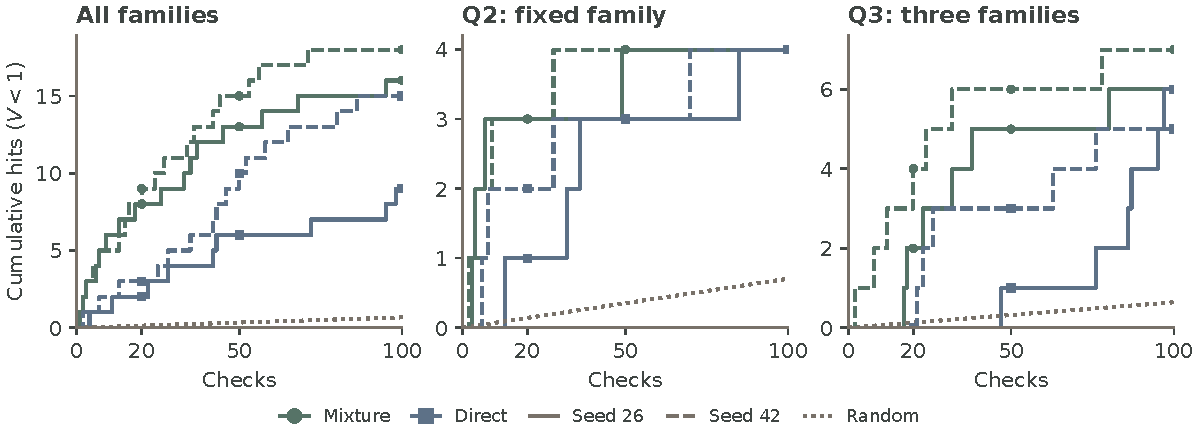
\includegraphics[width=\linewidth]{figures/screening.pdf}
\caption{Cumulative $V<1$ hits on file 03. Circles indicate the mixture, squares direct regression, solid lines seed 26 and dashed lines seed 42. The dotted line gives the expected cumulative count under random selection.}\label{fig:allbudgets}
\end{figure}
\subhead{Family choices for the blind candidate}
For the blind finalist, fixing La on A and Ti on B leaves three distinct compositions in the Q3 pool. Their anion fractions, in the order O, N, F, are $(1,0,0)$, $(2/3,1/3,0)$ and $(2/3,0,1/3)$. Equation~\eqref{eq:envelope} takes the minimum over these three discrete alternatives. Figure~\ref{fig:families} compares their stoichiometry and frozen scores. The data give no site-resolved geometry for the blind material.

\begin{figure}[htbp]
\centering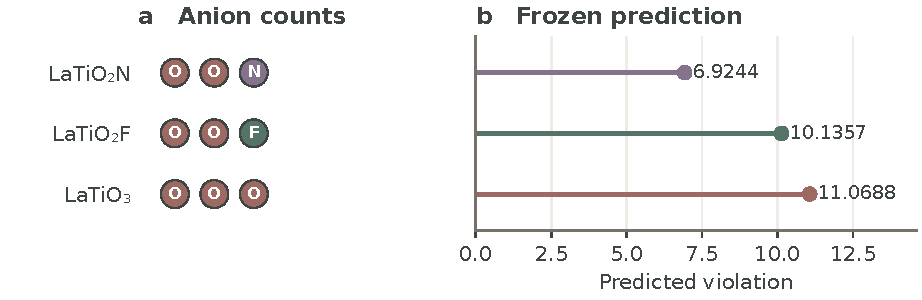
\includegraphics[width=\linewidth]{figures/anion_substitution.pdf}
\caption{Three anion compositions for the same La--Ti pair. Symbols count anions per formula unit. Predictions come from the refitted Q3 score table. The physical violation of the blind recommendation remains unknown.}\label{fig:families}
\end{figure}

The three minima share Ti on the B site and differ at A. They are $(\mathrm{Sn},\mathrm{Ti})$ at 3.268113 in O3, $(\mathrm{La},\mathrm{Ti})$ at 6.924382 in NO2, and $(\mathrm{Ca},\mathrm{Ti})$ at 4.585642 in FO2. Eight of the ten lowest scores across the full three-family pool also place Ti at B. This concentration describes the frozen surrogate. The ten records are selected extremes and cannot establish a general causal effect of Ti.

Holding La and Ti fixed, switching from NO2 to FO2 increases the score from 6.9244 to 10.1357, and switching to O3 raises it to 11.0688. Across all 2,704 pairs, however, O3 supplies the smallest score in 2,188 cells, NO2 in 378 and FO2 in 138. Each cell has a unique family minimum in the stored table. Thus choosing the family with the most pairwise wins would overlook the preferred family for the blind finalist.

The public Q3 winner also allows a physical check. Its formation energy of 0.10 eV, gap of 2.50 eV and VBM of 6.998833 eV all pass the corresponding thresholds. Its CBM of 4.518833 eV exceeds 4.50 by only 0.018833 eV, accounting for its entire reported violation. For the blind $\mathrm{LaTiO_2N}$ candidate, only composition and surrogate rank are observed. A new physical calculation would be needed to identify its limiting property.

\FloatBarrier
\lstset{language=Python,basicstyle=\fontsize{8.5}{10}\selectfont\ttfamily,
  columns=fullflexible,keepspaces=true,breaklines=true,breakatwhitespace=false,
  frame=none,backgroundcolor=\color{white},rulecolor=\color{white},
  keywordstyle=\color{black},stringstyle=\color{black},commentstyle=\color{black!65},
  aboveskip=2pt,belowskip=4pt,showstringspaces=false}
\newcommand{\program}[2]{\par\addvspace{1.2\baselineskip}\Needspace{8\baselineskip}\subhead{#1}\lstinputlisting{#2}}
\program{A1. Surrogate features and model components}{../exploration/compare_surrogates.py}
\program{A2. Source checks and label reconstruction}{../exploration/audit_data.py}
\program{A3. Withheld near-target and encoding experiments}{../exploration/test_innovation_ideas.py}
\program{A4. Physical-property-first prediction}{../exploration/compare_physical_properties.py}
\program{A5. Whole-grid SDK precision audit}{../exploration/audit_sdk_precision.py}
\program{A6. Frozen predictions and grouped folds}{screen.py}
\program{A7. Integer QUBO construction, exact solution and checks}{solve.py}
\program{A8. Manuscript figures}{figures.py}
\program{A9. Measured values for the manuscript tables}{tables.py}
\program{A10. Crystal geometry and screening diagnostics}{material_figures.py}
\program{A11. Perovskite structure, band edges and anion compositions}{perovskite_plates.py}
\program{A12. Gap-gate replay and validation ablation}{gate_audit.py}
\program{A13. Consistency and margin diagnostics}{mechanisms.py}
\program{A14. Weighted gate and QUBO readout}{crystal_scenes.py}
\program{A15. Direct-regression capacity controls}{capacity_audit.py}

\end{document}
